\subsection{Applications}
\label{sec:application}


\begin{figure*}[t]
	\centering
	\subfloat[Scalability.\label{fig:kv_scalability}]
	{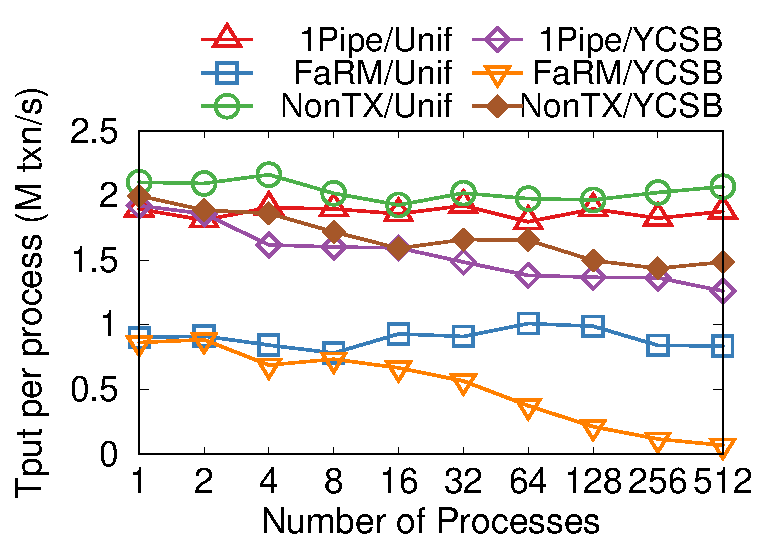
\includegraphics[width=.32\textwidth]{gnuplot/kv_scalability.eps}}
	\hspace{0.01\textwidth}
	\subfloat[Average latency of YCSB workload.\label{fig:kv_latency_ycsb}]
	{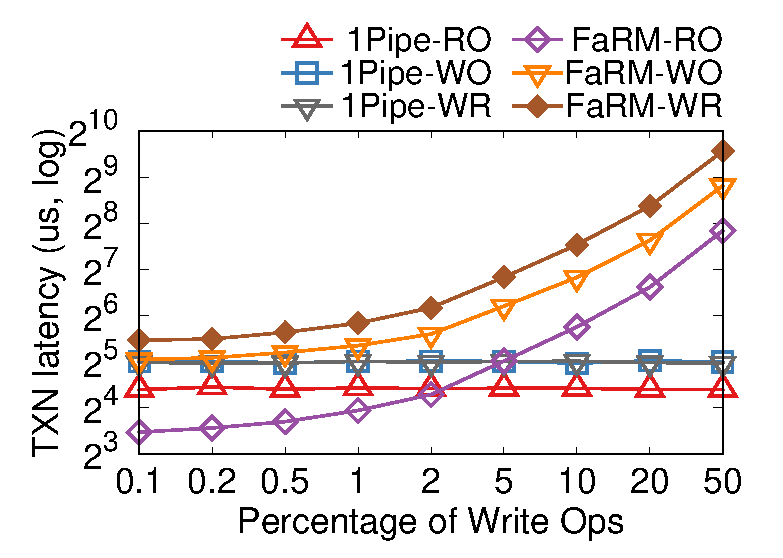
\includegraphics[width=.32\textwidth]{gnuplot/kv_latency_ycsb.eps}}
	\hspace{0.01\textwidth}
	\subfloat[Different transaction sizes.\label{fig:kv_multikey}]
	{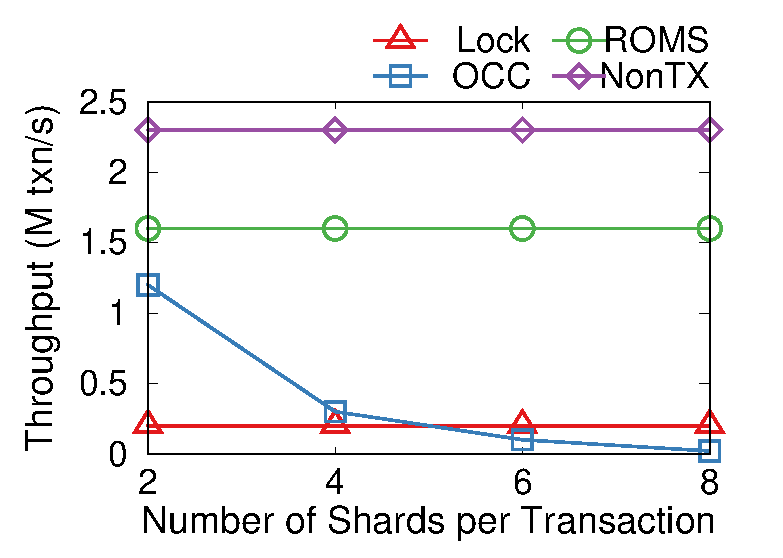
\includegraphics[width=.32\textwidth]{gnuplot/multishard.eps}}
	\caption{Performance of a transactional key-value store.}
	\vspace{-15pt}
\end{figure*}


\subsubsection{Transactional Key-Value Store}
\label{subsec:eval-kvs}


We evaluate a distributed transactional key-value store where each server process stores a portion of KVs in memory without replication using C++ \textit{std::unordered\_map}.
A transaction (TXN) is composed of multiple independent KV read or write operations.
%We use the same number of TXN initiator and server processes.
TXN initiators dispatch KV operations to server processes by hash of key.
Read-only (RO) TXNs are served by best effort \sys{}, while read-write (WR) and write-only (WO) TXNs use reliable \sys{}.
For comparison, we implement non-replicated and non-durable FaRM~\cite{dragojevic2014farm} which serves RO TXNs in 1 RTT by reading the KVs and checking lock and version. WR and WO TXNs in FaRM use OCC~\cite{kung1981optimistic} and two-phase commit.
As a theoretical performance upper bound, we also compare with a non-transactional system.

Each TXN has 2 KV ops by default, where read and write are randomly chosen for each op.
Keys are 64-bit integers generated either uniformly random or by Zipf distribution in YCSB~\cite{cooper2010benchmarking}. YCSB has hot keys.
The value size is randomly generated according to Facebook's ETC workload~\cite{atikoglu2012workload}.
We record average TXN latency at 95\% of peak throughput.


In Figure~\ref{fig:kv_scalability}, 50\% of TXNs are read-only.
In both uniform and YCSB distribution, \sys{} delivers scalable throughput (per-process throughput does not degrade), which is 90\% of a non-transactional key-value store (NonTX).
As number of processes increase, YCSB scales not as linearly as uniform, because contention on hot keys lead to load imbalance of different servers.
With 512 processes, YCSB has 70\% throughput of uniform both for \sys{} and NonTX.
In uniform workload that is free of contention, FaRM delivers 50\% throughput of \sys{} because WR and WO TXNs need 3 or 4 RTTs.
In YCSB workload, FaRM does not scale because it \emph{locks} keys for 2 RTTs during WO/WR TXN commit, and the hot keys block all conflicting TXNs.
In contrast, \sys{} does not lock keys. Each server processes TXNs on a same key in order.

In Figure~\ref{fig:kv_latency_ycsb}, we adjust the percentage of write ops and measure latency of RO, WO, and WR TXNs with 512 processes.
The latency of \sys{} is almost constant because servers process read and write ops on a same key in order. WO and WR use reliable \sys{}, which is slower than RO that uses best effort \sys{}.
For pure RO workload, FaRM has lower latency than \sys{} because it completes in 1 RTT and does not wait for network-wide reorder.
Non-contended FaRM WO and WR consumes 3 and 4 RTTs, respectively, which is slightly worse than \sys{}.
However, with high write percentage, FaRM latency skyrockets due to lock contention on hot keys and TXN aborts due to inconsistent read version.

In Figure~\ref{fig:kv_multikey}, we alter the number of keys per TXN, and measure total KV op/s with 512 processes.
95\% of TXNs are read-only.
\sys{} and NonTX are agnostic of TXN size because their throughputs are only bounded by CPU processing and network messaging rate.
With a low write percentage (5\%), FaRM/YCSB delivers 40\% throughput of \sys{} with 2 KV ops per TXN, but the performance plummets with larger TXN size, because TXN abort rate increases with the number of keys in a TXN.

%\textbf{Write percentage - RO / WO / WR Latency - Uniform.}

%\textbf{Write percentage - Throughput - Uniform/YCSB. Expect: straight line vs. drop for high update percentage in FaRM (higher overhead). Not good, affect throughput due to different ops.}

\iffalse
FaRM RO latency = RTT / RO success rate
RO success rate = both objects are unlocked; value write version not broken.
FaRM WO latency = RTT * 3 (write, prepare + lock, commit + unlock) / WO success rate
WO success rate = write lock succeed.
FaRM WR latency = RTT * 4 (read/write, prepare + lock, validate, commit + unlock) / WO success rate
WR success rate = write lock succeed; read version correct.
\sys{} RO latency = RTT + best-effort reordering delay $\approx$ 2 RTT
\sys{} WR/WO latency = RTT + reliable reordering delay $\approx$ 3 RTT
NonTX latency = RTT

\sys{} / NonTX throughput: unchanged.
\sys{}  = NonTX / 1.1 due to additional round-trip in reliable.
FaRM throughput: NonTX / ((1/RO success rate + 1.4/WR success rate + 1.3/WO success rate) / 3).

50\% are read-only TXNs, 50\% are read-write TXNs.
\fi


%\textbf{Number of KVs per TXN - Throughput - YCSB/Uniform. Expect: reverse proportional with number of objects, but NonTX and \sys{} are similar. More objects, higher contention rate.}



%\textbf{YCSB skewness - Throughput (50\% GET, 2 objects). Expect: in skewed workload, locking has higher transaction collision rate.}

%\textbf{YCSB skewness - Latency (50\% GET, 2 objects). Expect: slight increase in latency vs. high increase in latency due to aborts.}

%As a case study, we study the transaction performance of transactional key-value stores under YCSB+T~\cite{dey2014ycsbt} skewed workload.
%For the sake of simplicity, we focus on single round-trip (one-shot) transactions. Single-node transactions can be serialized on the server at the current timestamp, thus do not need \sys. General transactions with predetermined read and write sets can be reduced to single round-trip transactions, by sending the read and write set to each shard via \sys. During further execution of a general transaction, each shard can track the dependency and execute the read and write operations in timestamp order.

%Figure~\ref{fig:ycsb} shows the throughput and latency, where each atomic operation accesses two randomly chosen objects.
%\sys achieves 6.4~M transactions per server (0.8~M transactions per core) with 40~$\mu$s latency, close to an non-atomic system (NonTX) where operations are scattered directly without ordering.
%The throughput gap between \sys and NonTX is mainly due to CPU processing of reordering messages.
%The latency gap originates from the reordering delay.
%In comparison, the throughput of locks is limited by RTT.
%The throughput of centralized coordination is bottlenecked by the coordinator.

%Figure~\ref{fig:multishard} compares the single-core transaction throughput with an increasing number of keys per atomic scattering.
%Now we consider other timestamp-based methods.
%With more keys per scattering, the chance of transaction abort increases, because reordering in any one of the keys would cause transaction abort.

%Figure~\ref{fig:multishard} compares the throughput of TOMS, OCC, lock-based and non-transactional key-value stores.
%Each transaction accesses 8 unique remote objects.
%If the 8 objects are on two shards, OCC has 50\% chance of transaction abort, so the throughput is 50\% of non-transactional systems. When the objects are distributed on more shards, OCC has an exponentially higher chance of abort (Sec.~\ref{sec:toms}). The throughputs of other systems are unrelated to number of shards. \sys has 10x transaction throughput than lock-based systems, as well as OCC systems with more than 4 shards per transaction. The throughput of \sys is close to the theoretical bound of non-transactional system.

\iffalse
Finally, we study the efficiency of our loss detection and recovery mechanism in Sec.~\ref{sec:lossy}.
Assume 1/10 of the transactions have conflicts, \textit{i.e.}, if a transaction is rollbacked, 1/10 of uncommitted transactions also need rollback.
Figure~\ref{fig:ycsb-loss} simulates the transaction throughput and latency under different loss ratios.
With reliable \sys, packet loss is transparent to applications, and the transaction throughput is approximately the network goodput.
If \sys does not handle packet loss, the transaction processing application needs to rollback all uncommitted transactions on packet loss.

On the latency side, reliable \sys adds one RTT of latency to derive the delivery barrier.
If any packet is lost, reliable \sys needs to wait for an additional RTT to retransmit the packet.
When packet loss is rare, as in most data center networks, handling loss by applications provides lower latency.
Under high packet loss probability, however, handling losses in \sys is better.
\fi

\iffalse
\begin{figure}[t]
\centering

\includegraphics[width=0.3\textwidth]{images/fixme.pdf}
\caption{[Testbed] Comparing YCSB+T throughput on inter-DC WAN.}
\vspace{-10pt}
\label{fig:ycsb-inter-dc}
\end{figure}

Figure~\ref{fig:ycsb-inter-dc} compares the throughput of cross-datacenter workload of TOMS and lock-based.
\fi

\begin{figure*}[t]
    \begin{minipage}[]{.66\textwidth}
    	\centering
    	\subfloat[Scalability.\label{fig:tpcc-combined}]
    	{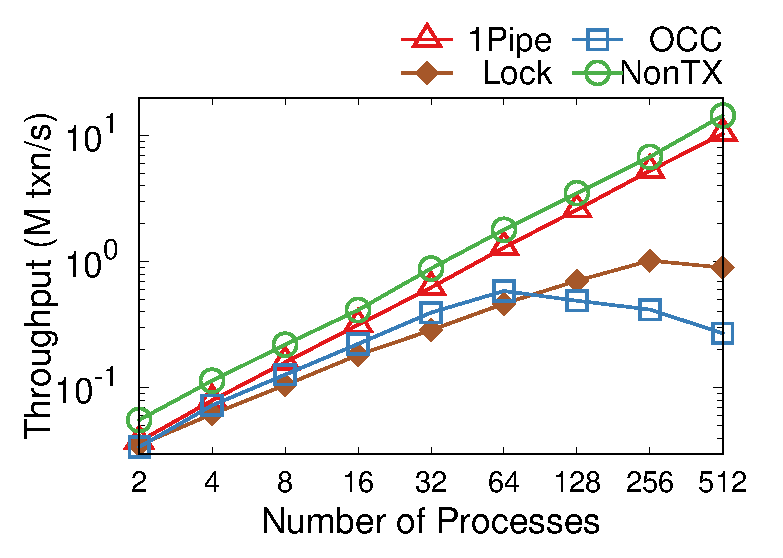
\includegraphics[width=.49\textwidth]{gnuplot/tpcc-combined.eps}}
    	\hspace{0.01\textwidth}
    	\subfloat[Resilience of packet loss.\label{fig:tpcc-loss}]
    	{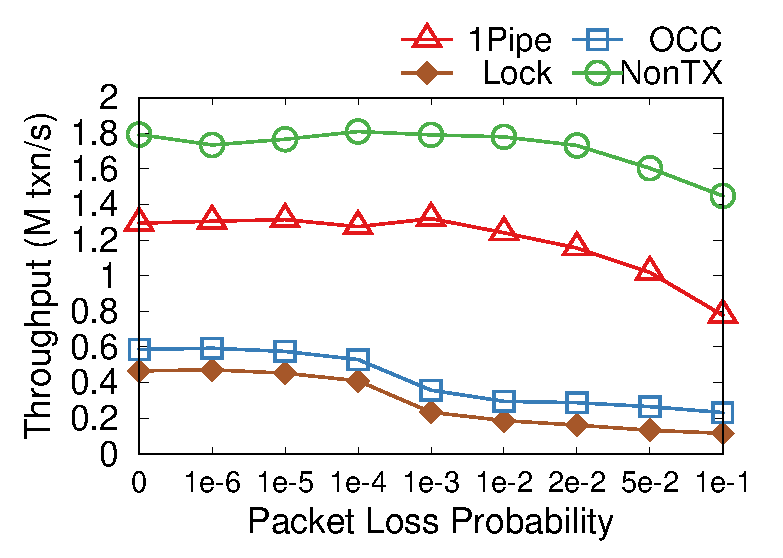
\includegraphics[width=.49\textwidth]{gnuplot/tpcc-loss.eps}}
    	\caption{TPC-C transaction benchmark.}
    	\label{fig:tpc-c}
    \end{minipage}
    \hspace{0.01\textwidth}
    \begin{minipage}[]{.32\textwidth}
        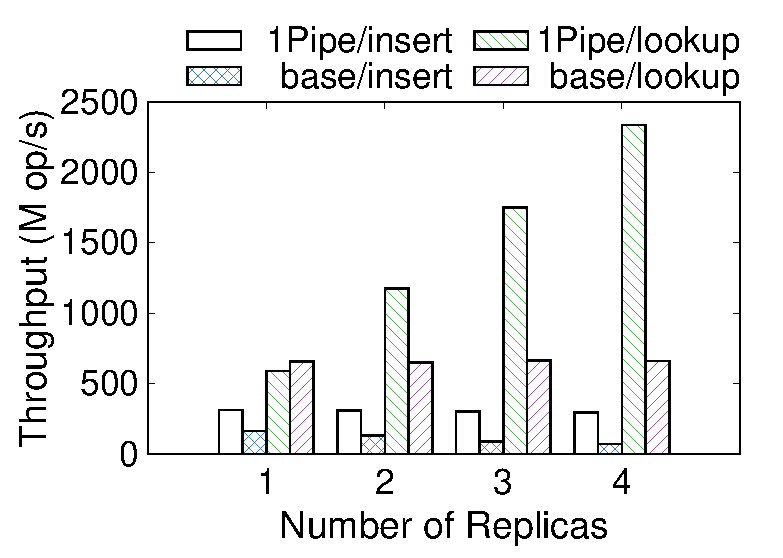
\includegraphics[width=\textwidth]{gnuplot/remote-hashtable.eps}
    	\caption{Per-client throughput of a replicated remote hash table.}
    	\label{fig:remote-hashtable}
    \end{minipage}
    \vspace{-15pt}
\end{figure*}

\iffalse
\begin{figure*}[t]
	\centering
	\subfloat[New-Order 50\%, Payment 50\%.\label{fig:tpcc-combined}]
	{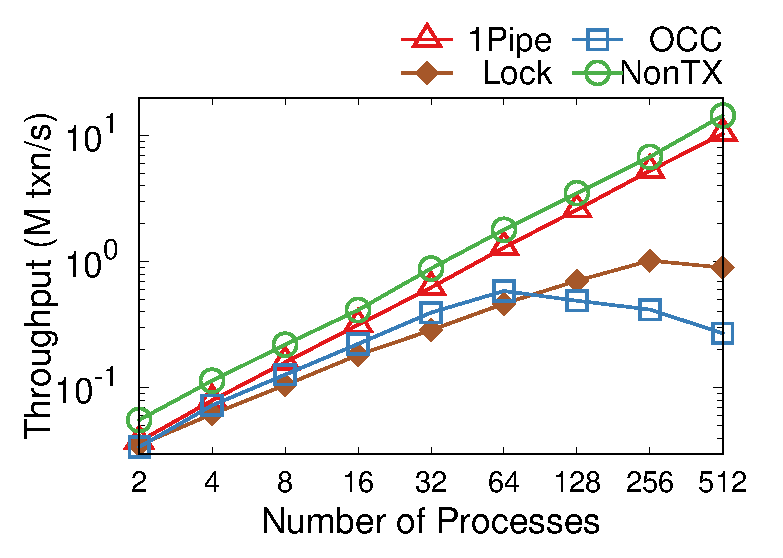
\includegraphics[width=.3\textwidth]{gnuplot/tpcc-combined.eps}}
	\hspace{0.02\textwidth}
	\subfloat[Payment 100\%.\label{fig:tpcc-payment}]
	{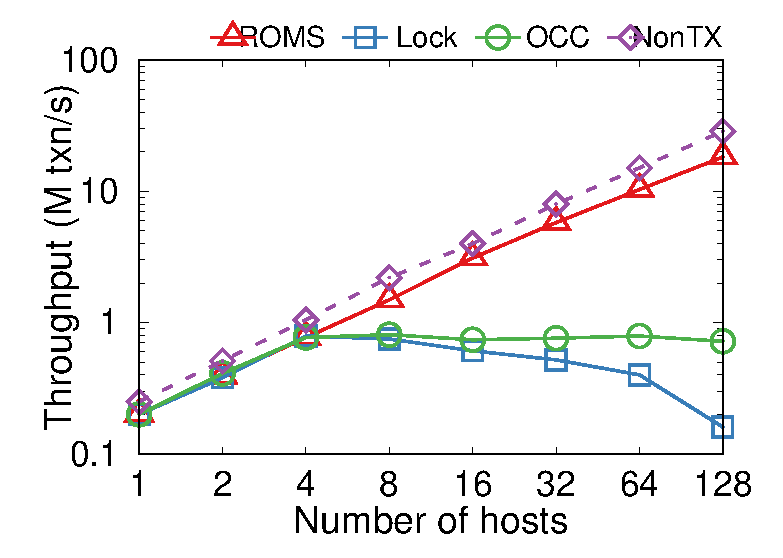
\includegraphics[width=.3\textwidth]{gnuplot/tpcc-payment.eps}}
	\hspace{0.02\textwidth}
	\subfloat[New-Order 100\%.\label{fig:tpcc-neworder}]
	{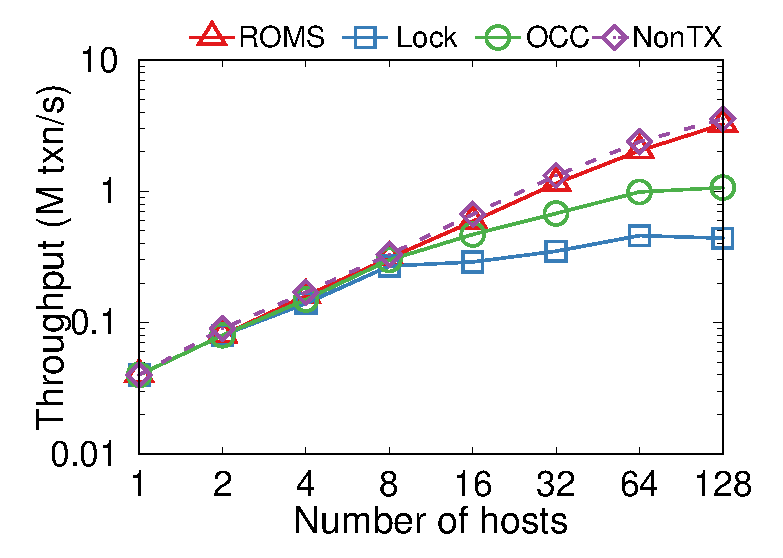
\includegraphics[width=.3\textwidth]{gnuplot/tpcc-neworder.eps}}
	\caption{TPC-C benchmark with 4 warehouses.}
	\label{fig:tpc-c}
	\vspace{-10pt}
\end{figure*}
\fi

\subsubsection{Independent General Transactions}
\label{subsec:eval-transactions}

We apply \sys to independent general TXNs (Sec.\ref{subsec:dao}).
We benchmark New-Order and Payment TXNs in TPC-C~\cite{tpcc}, which constitute 90\% of TPC-C workload.
For simplicity, we do not implement non-independent TXNs in TPC-C, which should fall back to traditional concurrency control mechanisms.
We use 4 warehouses which are stored in-memory with 3 replicas.
Concurrency control and replication are implemented with a batch of commands sent to all shards and replicas, similar to Eris~\cite{eris} but replaces its central sequencer with timestamps.
We assume TXNs never abort.
As shown in Figure~\ref{fig:tpcc-combined}, two-phase locking (2PL) and OCC do not scale, because each Payment TXN updates its corresponding warehouse entry and each New-Order reads it~\cite{yu2014staring}, leading to 4 hot entries.
The throughput of OCC and 2PL reaches peak at 256 and 64 processes, respectively. With more processes, the throughput becomes lower~\cite{mu2014extracting}.
%When conflicts are few, OCC is better; with more conflicts, 2PL is better~\cite{mu2014extracting}.
In contrast, \sys{} scales linearly with number of processes. With 512 processes, \sys achieves 10.35M TXNs per second, which is 71\% of a non-transactional baseline system, 10x of lock and 17x of OCC. %With more processes, \sys{} would be bounded by CPU processing capacity of contended entries.

Figure~\ref{fig:tpcc-loss} shows TXN throughput under different simulated packet loss rates.
We fix process number to be 64.
With \sys{}, although packet loss affects TXN latency (not measured in TPC-C, but should be similar to Figure~\ref{fig:reorder-loss}), the impact on throughput is insignificant. %because the network is fully utilized to transmit new TXNs during retransmission.
However, in 2PL and OCC commit, a locked object cannot be released until the TXN completes, so, TXN throughput under contention is inversely proportional to TXN latency.
TXN latency increases with packet loss rate because replicas wait for the last retransmitted packet to maintain sequential log ordering.

Finally, we evaluate failure recovery of replicas by disconnecting the physical link of a host. \sys{} detects failure and removes the replica in $181 \pm 21 \mu$s. The affected TXNs are aborted and retried, with an average delay of $308 \pm 122 \mu$s. It is much faster than using application heartbeats to detect failures, which takes milliseconds. After the link reconnects, the replica synchronizes log from other replicas in 25 ms.

\subsubsection{Remote Data Structures}
\label{subsec:data-structure}

\sys{} can remove ordering hazards in remote data structure access (Sec.\ref{subsec:order-hazards}).
We implement a distributed concurrent hash table that uses a linked list to store key-value pairs (KVs) in a same hash bucket. The hash table is sharded on multiple servers.
Different from Sec.\ref{subsec:eval-kvs} where servers process KV ops, in this section, clients access the remote hash table using RDMA \emph{one-sided} read, write, and CAS.
The baseline system uses leader-follower replication.
16 clients lookup or insert uniformly random keys in parallel.

As Figure~\ref{fig:remote-hashtable} shows, without replication, \sys{} improves per-client KV insertion throughput to 1.9x because \sys{} removes the \emph{fence} between writing KV pair and updating the pointer in hash bucket.
KV lookup throughput reduces by 10\%, due to additional reordering delay.
If the hash table is replicated traditionally, a write op is sent to the leader, which involves CPU software to replicate to followers.
With 3 replicas, \sys{} improves KV insertion throughput to 3.4x.
In \sys{}, all KV operations are ordered by timestamp, so all replicas can serve lookup requests, and the throughput scales with number of replicas.
In contrast, with leader-follower replication, to maintain serializability of reads and writes, only the leader can serve lookups.


\subsubsection{Replication in Distributed Storage}
\label{subsec:ceph}

We apply \sys{} to Ceph~\cite{weil2006ceph} distributed storage. Ceph OSD uses a primary-backup replication scheme, where the backups are also written sequentially. With 3 replicas, a client waits for 3 disk writes and 6 network messages (3 RTTs) in sequence. With reliable \sys{}, the client can write 3 replicas in parallel, thus the end-to-end write latency is reduced to 1 disk write and 1 RTT. Experiment shows that in an idle system with Intel DC S3700 SSDs, the latency of 4KB random write reduces from $160 \pm 41 \mu$s to $58 \pm 28 \mu$s (64\% reduction).


%\subsection{Multiple Round-Trip Transactions}

%TPC-C transaction benchmark

%Compare transaction throughput with Eris, TAPIR, DrTM+R (lock based), OCC and theoretical optimal (non-transactional)

%\subsection{Coordination-Free Causal Ordering}

%Our barrier timestamp is guaranteed to be lower than data timestamp, so if we send a message A after receiving a message B, A has higher timestamp than B. This can ensure ordering of events in a distributed system. For example, client A sends a command W to write database D, then sends a message to client B. When B receives the message from A, it sends command R to read database D. In our system, the database read command R is guaranteed to be processed after the write command W, so no additional synchronization is needed.